\section{Results}
\label{sec:results}
In this section we describe the results obtained from our simulations. We have simulated two scenarios: A square room where the pedestrians exit throw a single door, and pedestrians walking throw a corridor where there is a bidirectional flow. For each scenario we describe the parameters we have set for the scenario, which features we found worth measuring for this scenario, the results we expected, and the results we obtained. Possible remedies for any discrepancies between the expected and the actual results are discussed in section~\ref{sec:discrepancies}.

\subsection{The square room scenario}
In this scenario we simulate pedestrians leaving a square room of 10 m by 10 m with a single $80cm$ wide door. 100 pedestrians are positioned randomly throughout the room. The second the simulation start all pedestrians head for the exit. The parameters for this simulation are as follows:
\begin{itemize*}
    \item $A: 2,2$, $B: 0,2$, $U: 2.0$, $\lambda: 0,1$.
    \item Mean desired velocity: $1,34 m/s$, deviation $0,26 m/s$. Max velocity factor $1,3$.
    \item Radius mean $0,3 m$, deviation $0,01 m$.
    \item Relaxation time: $1,0 s$.
    \item Number of pedestrians: $100$.
\end{itemize*}

First the claim of the "faster-is-slower" effect is tested.
\begin{quote}
Even counterintuitive
effects are well reproduced. This includes the “faster is-
slower effect” and stripe formation in intersecting flows. \cite{self-org}
\end{quote}
We would then expect that a high nervousness would lead to slower evacuation, because of additional clogging at the doorway. But this phenomena do not occur in our simulation see figure \ref{FastIsSlow}
%\begin{figure}
%\centering
%\includegraphics[scale=1]{FastIsSlowNot}
%\end{figure}
The larger the nervousness the faster is the evacuation. We have increased the max-velocity factor sow much that people eventually move throw the walls. This start occurring around max-velocity-factor = 2.5, and measurements beyond this point are neglected.

Pedestrian flow rate is measure in the door opening, and the density of pedestrians in a 2 m by 2 m area directly in front of the door is measured. We also measure the time it takes for all pedestrians to leave the room.

The parameters for this simulation are as follows:

% TODO: Add parameters that are varied.


\subsection{The corridor scenario}
In this scenario we simulate pedestrians walking in both directions along a 20 
m long and six metres wide corridor. The pedestrians are divided into two 
groups, starting in opposite ends of the corridor and moving towards each 
other. The targets the pedestrians move towards are set 500 metres to each 
side, to make pedestrians walk in almost a straight line instead of converging 
towards the middle of the corridor. Flow rate is measured in the middle of the 
corridor, as is density. We start out with 100 pedestrians, adding a 
continuous inflow of three pedestrians per second, to simulate people arriving 
from outside the simulated area. Both the initial placement and the inflow of 
pedestrians are distributed randomly (i.e. approximately evenly) between the 
two ends of the corridor.

We expect to see lane formations through out our simulations
and the freezing by heating effect when we start raising the mean velocity
of the agents.
In the first simulation the parameters are set after \cite{ABconstant} and
\cite{self-org}, to see if we can replecate their simulations and results.
The parameters for this simulation are as follows:

\begin{itemize*}
    \item $A: 2,2$, $B: 0,2$, $U: 2,0$, $\lambda: 0,1$.
    \item Mean desired velocity: $0,74 m/s$, deviation $0,26 m/s$. Max 
        velocity factor $1,3$.
    \item Radius mean $0,3 m$, deviation $0,01 m$.
    \item Relaxation time: $1,0 s$.
    \item Number of pedestrians: $20$ starting, adding $1/s$.
\end{itemize*}

When running the simulation we observe lane formations, and they almost clog up
in the corridor.

To get the freezing by heating effect we raise the max desired velocity to 4.
The other parameters are fixed:

\begin{itemize*}
    \item $A: 2,2$, $B: 0,2$, $U: 2,0$, $\lambda: 0,1$.
    \item Mean desired velocity: $0,74 m/s$, deviation $0,26 m/s$. Max 
        velocity factor $4,0$.
    \item Radius mean $0,3 m$, deviation $0,01 m$.
    \item Relaxation time: $1,0 s$.
    \item Number of pedestrians: $20$ starting, adding $1/s$.
\end{itemize*}

When we do a simulation with the max velocity factor set to $4.0$, the clogging
that occurs in the beginning eases up, and the pedestrians relatively fast
get out of the clogging and continuous toward their target.

\begin{figure}
\centering
\subfloat[The figure show the density in corridor when the parameters are set as \cite{ABconstant} and \cite{self-org}.]{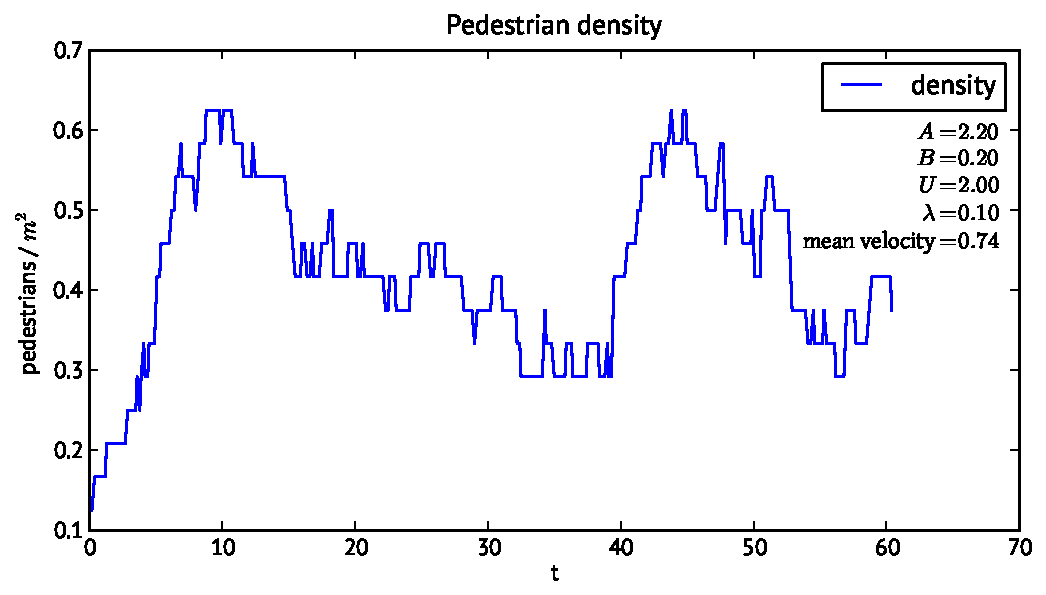
\includegraphics[scale=0.45]{Figures/dens_init_20.pdf}}
\subfloat[This figure shows the density in the corridor when the max velocity factor is set to $4.0$, and the other parameters as figure a.]{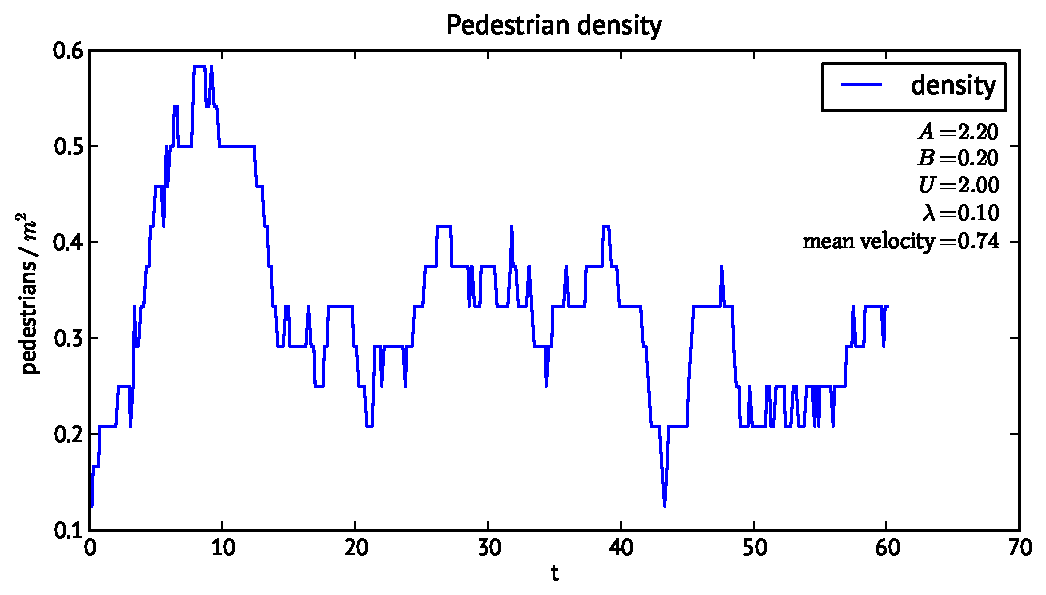
\includegraphics[scale=0.45]{Figures/dens_mvel4_20.pdf}}
\caption{These figures was made to see if the freezing by heating effect when raising the max velocity factor. As seen in the figures, the
density does not increase when the max desired velocity is increased. When raising the max desired velocity the density gets lower because
the pedestrians more easely get through the crowd.}
\label{fig:freezingbyheating}
\end{figure}

\cite{helbing00} set the relaxation time to $0,5$. As the first corridor simulations we set the parameters as \cite{ABconstant}
and then change the relaxation time to $0,5$ as \cite{helbing00}. After the simulation with the initial conditions, we raise the
max desired velocity to see if we can replicate the freezing by heating effect.

The initial simulation has the following parameters:

\begin{itemize*}
    \item $A: 2,2$, $B: 0,2$, $U: 2,0$, $\lambda: 0,1$.
    \item Mean desired velocity: $0,74 m/s$, deviation $0,26 m/s$. Max 
        velocity factor $1,3$.
    \item Radius mean $0,3 m$, deviation $0,01 m$.
    \item Relaxation time: $0,5 s$.
    \item Number of pedestrians: $20$ starting, adding $1/s$.
\end{itemize*}

The next simulation the parameters are as follows:

\begin{itemize*}
    \item $A: 2,2$, $B: 0,2$, $U: 2,0$, $\lambda: 0,1$.
    \item Mean desired velocity: $0,74 m/s$, deviation $0,26 m/s$. Max 
        velocity factor $4,0$.
    \item Radius mean $0,3 m$, deviation $0,01 m$.
    \item Relaxation time: $0,5 s$.
    \item Number of pedestrians: $20$ starting, adding $1/s$.
\end{itemize*}

When comparing the simulations we do not see the freezing by heating effect.
Instead we see that the pedestrians more easely escape the clogging, and the flow in each directions
gets more steady.

\begin{figure}
\centering
\subfloat[The figure show the density in corridor when the parameters are set as \cite{ABconstant} and \cite{helbing00}.]{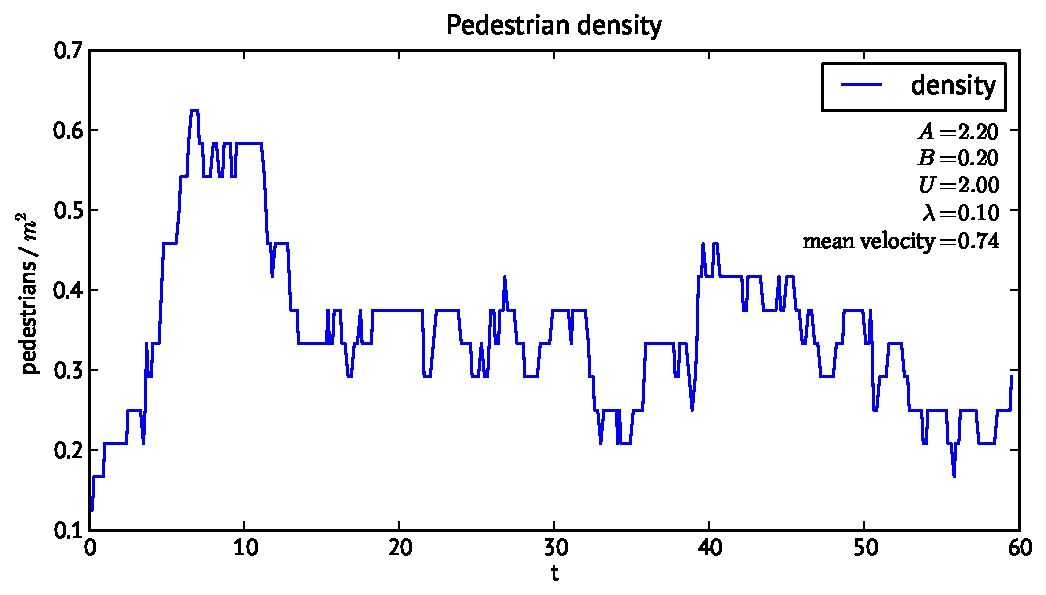
\includegraphics[scale=0.45]{Figures/dens_relax05_20.pdf}}
\subfloat[This figure shows the density in the corridor when the max velocity factor is set to $4.0$ and the max desired velocity is set to $4,0$, and the other parameters as figure a.]{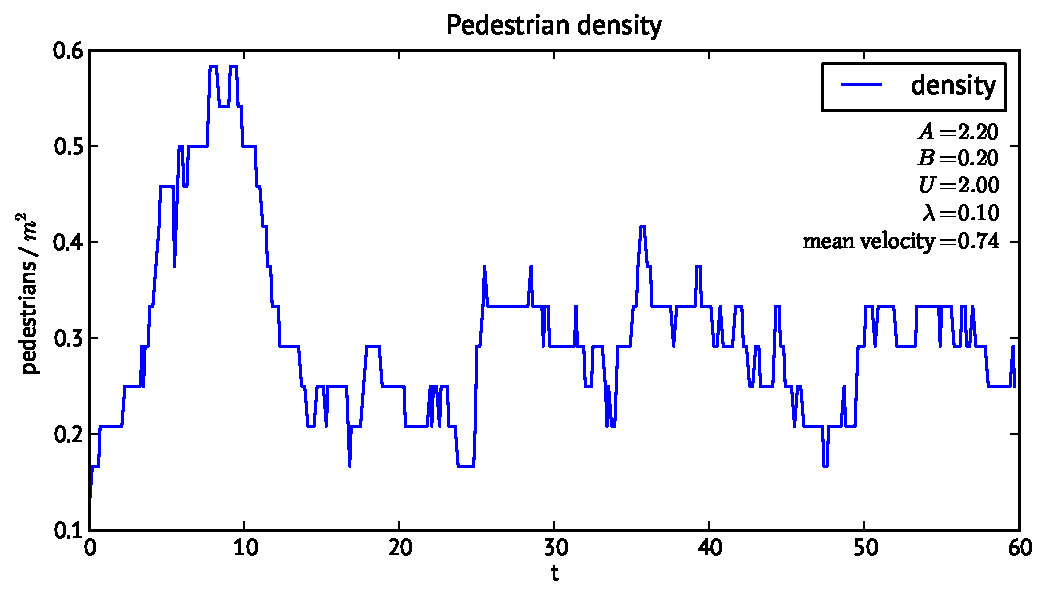
\includegraphics[scale=0.45]{Figures/dens_relax05_mvel4_20.pdf}}
\caption{These figures was made to see if the freezing by heating effect when raising the max velocity factor. As seen in the figures, the
density does not increase when the max desired velocity is increased. When raising the max desired velocity the density gets lower because
the pedestrians more easely get through the crowd.}
\label{fig:freezingbyheating}
\end{figure}


% TODO: Add parameters that are varied.
